% !TEX TS-program = lualatex
% !TEX encoding = UTF-8

\documentclass[Session2026.tex]{subfiles}

\ifcsname preamble@file\endcsname
  \setcounter{page}{\getpagerefnumber{M-10_appendice}}
\fi

\begin{document}

\addcontentsline{toc}{chapter}{Appendice}
\restoregeometry
\vspace*{2cm}

\bigtitle{Te Deum}{Appendice}{Te Deum}
\smalltitle{ton monastique}
\gscore{hy_te_deum}

\newpage

\bigtitle{Ave Maris Stella}{Appendice}{Ave Maris Stella}
\smalltitle{ton solennel}
\gscore{hy_ave_maris_stella}

\pagebreak

\null\vfill

\bigtitle{Tons des psaumes}{Appendice}{Tons des psaumes}
\smalltitle{selon l'office monastique rénové}

\smalltitle{Ton 1}
\incipit{ton}{1}

\smalltitle{Ton 2}
\incipit{ton}{2}

\newpage

\smalltitle{Ton 2*}
\incipit{ton}{2s}

\smalltitle{Ton 3}
\incipit{ton}{3}

\smalltitle{Ton 4}
\incipit{ton}{4}

\newpage

\smalltitle{Ton 4*}
\incipit{ton}{4s}

\smalltitle{Ton 5}
\incipit{ton}{5}

\smalltitle{Ton 6}
\incipit{ton}{6}

\newpage

\smalltitle{Ton 7}
\incipit{ton}{7}

\smalltitle{Ton 8}
\incipit{ton}{8}

\smalltitle{Ton C, ou «in directum»}
\incipit{ton}{C}

\newpage 

\smalltitle{Ton D}
\incipit{ton}{D}

\smalltitle{Ton E, ou «irrégulier»}
\incipit{ton}{E}

\smalltitle{Ton «pérégrin»}
\incipit{ton}{P}

\newpage

\bigtitle{Commentaires de pièces}{Appendice}{Commentaires de pièces}

\setlength{\parindent}{10mm}
\setlength{\parskip}{2.5mm}

\smalltitle{Introitus • Suscepimus Deus}

Nous célébrons cette semaine la XIV\textsuperscript{e} semaine du Temps ordinaire. 
L'introït choisi par l'Église pour célébrer ce temps est le \emph{Suscepimus Deus}, 
c'est le même chant d'entrée que celui de la
Présentation du Seigneur. Le texte de cet introït est tiré du Psaume
XLVII, versets 10 et 11, hymne dans lequel le priant exprime son immense
gratitude à Dieu pour les innombrables grâces qu'il a reçues de Lui.
Tout d'abord, pour le don de son Esprit qui a mis en nous la vie divine
et qui la soutient et nous encourage, par son action incessante, à la
vivre pleinement... Et bien sûr, par toutes les autres choses que
chacun de nous, au plus profond de son être, connaît et reconnaît comme
des «~dons~» du Très-Haut. \emph{Suscepimus, Deus, misericordiam tuam in
medio templi tui : secundum nomen tuum Deus, ita et laus tua in fines
terræ : justitia plena est dextera tua} - \emph{Nous avons reçu, ô Dieu,
ta miséricorde au milieu de ton temple ; avec ton nom, ô Dieu, ainsi ta
louange s'étend jusqu'aux extrémités de la terre ; ta droite est pleine
de justice.}

Ce texte est également utilisé pour le rite du début du noviciat dans
l'ordre bénédictin. Et, pour cette même raison, il a une valeur de
communion et de communauté qui est à l'origine de l'image du Temple et
de l'utilisation du pluriel du verbe \emph{Suscepimus}. C'est
l'assemblée liturgique qui reçoit le Seigneur, c'est toute la Communauté
qui rend grâce à Dieu d'avoir reçu sa miséricorde. Ce texte contient
également deux des attributs divins qui se complètent : la justice,
perfection de la volonté divine, et la miséricorde, pour laquelle nous
Le remercions. Ainsi, pour tout ce qui nous a été accordé, nous
remercions Dieu par ce chant de louange, un chant que nous voulons
porter \emph{jusqu'aux confins de la Terre} - \emph{in fines terræ}.

Quant à la mélodie, composée dans la majesté du 1er mode, elle chante
avant tout dans les hauteurs du mode, avec joie, avec une profonde
gratitude. L'intonation, caractéristique du 1er mode, va jusqu'à la
quinte agile et joyeuse, du RÉ, la tonique, au LA, la dominante :
\emph{suscépimus, Deus} - \emph{nous avons reçu, ô Dieu}. Cette joie
initiale se poursuit autour de la dominante dans les deux \emph{torculi}
de \emph{«~Deus~»}, LA-DO-LA, SOL-LA-SOL, une joie enveloppée d'une
grande révérence. Dans \emph{misericordiam tuam} - \emph{ta
miséricorde}, le mouvement mélodique atteint son apogée de cette
première phrase dans l'accent de \emph{«~misericordiam~»} avec ce
couronnement de la \emph{bivirga} sur le DO. De même, le mot
\emph{«~misericordiam~»} est enveloppé d'une ferveur reconnaissante, à
laquelle s'ajoute une touche de joie profonde et de gratitude sincère,
contagieuse, à l'adjectif possessif \emph{«~tuam~»}, magistralement mise
en valeur par un mouvement quilismatique, LA-SI-DO-LA, très expressif et
qui confère aussi, avec l'intervalle semitonal, SI-DO, cette proximité
et cette tendresse amoureuse à l'égard du Créateur. Dans la dernière
incise de cette première phrase, \emph{in medio templi tui} - \emph{au
milieu de ton temple}, une fervente révérence, une dévote adoration
s'installe clairement chez l'orant : dans le grave, le pieux
\emph{torculus resupinus} de l'accent de «~\emph{in medio~»},
FA-LA-FA-SOL ; dans l'aigu, le révérencieux \emph{porrectus flexus} avec
son saut de quarte à \emph{«~templi~»}, DO-LA-DO-SOL, auquel s'ajoute
dans \emph{«~tui~»} un autre motif mélodique pour amplifier cette
révérence totale, FA LA-SOL-FA-SOL-FA FA.

Dans la deuxième phrase, un changement s'opère : nous passons de
l'humble remerciement à la louange, de la cause à l'effet. Nous avons
remercié le Créateur pour tout ce que nous avons reçu, maintenant nous
le louons, nous le glorifions. D'autre part, nous sommes passés du nous,
\emph{«~suscepimus~»}, à un verbe à la troisième personne du singulier,
\emph{«~plena est~»}, qui fait référence à la justice divine. Il ne
s'agit plus de nous, qui avons reçu la grâce et l'amour de Dieu, mais de
Dieu lui-même. Dans \emph{secundum nomen tuum Deus} - \emph{comme ton
nom, ô Dieu}, la mélodie monte jusqu'au DO et y reste, c'est la note qui
domine, contrairement à la première phrase où elle se déplaçait entre le
FA et le LA. En effet, c'est le moment de la contemplation et de la
louange. Le locuteur regarde vers les hauteurs du mode, il cherche le
Seigneur, la louange éclate, lumineuse et enthousiaste. Notez le
mouvement jubilatoire des tierces dans \emph{«~secundum~»},
FA-LA(SOL)-DO. À \emph{«~nomen~»}, l'invocation du Nom éveille l'âme à
la contemplation de ce Nom, Dieu le Père, dans les hauteurs de la
mélodie. Le MI aigu est atteint dans l'accent de \emph{«~nomen~»}, puis
dans \emph{«~tuum~»} la mélodie revient au DO avec une \emph{tristropha}
contemplative qui souligne l'adjectif possesif (comme TON nom) avant de
chanter avec une pieuse révérence et de contempler le Seigneur dans
\emph{«~Deus~»} en dilatant le rythme dans un fervent \emph{pes
quadratus subbipunctis}, DO-RÉ-DO-LA LA.

Dans \emph{ita et laus tua} - \emph{ainsi ta louange}, l'admiration du
priant se poursuit, son désir s'exprime, avec fermeté et emphase, le DO
résonne fortement dans la \emph{bivirga} de l'accent de \emph{«~ita~»},
suivi d'un \emph{torculus} très révérencieux, DO-RÉ-LA, et d'une
\emph{clivis épisémée}, LA-SOL, qui met en valeur le mot
\emph{«~laus~»}, la louange. Dans \emph{«~tua~»}, nous assistons à l'un
des génies compositionnels de cette pièce : un mouvement quilismatique
solennel réapparaît, presque identique au \emph{«~tuam~»} de la première
phrase, seulement un peu plus développé dans l'aigu. Un lien
mélodico-verbal s'établit - cause à effet - nous recevons TA miséricorde
et donc TA louange résonne jusqu'aux extrémités de la terre. Dans
l'incise suivante, \emph{in fines terræ}, \emph{jusqu'aux extrémités de
la terre}, un bel arc mélodique couvre toute la terre, du DO aigu au MI,
avec deux magnifiques sauts, l'un de tierce, DO-LA, et l'autre de
quarte, DO-SOL. En outre, nous trouvons un autre des génies
compositionnels de cette pièce : le compositeur utilise la même tournure
mélodique que \emph{templi tui} pour \emph{fines terræ} : la louange et
la révérence que nous présentons au Seigneur n'ont pas seulement lieu
dans son saint Temple, physiquement, dans le Temple, mais aussi dans
toutes les extrémités de la terre et dans notre Temple intérieur, notre
âme.

La pièce se termine par un retour à l'ambitus grave : \emph{justitia
plena est dextera tua} - \emph{ta main droite est pleine de justice}.
Mais ce n'est plus l'atmosphère joyeuse du début ; elle devient
paisible, elle prend de la sérénité et de la fermeté. Après la
contemplation des «~merveilles de Dieu~», il y a eu la joyeuse
jubilation. Mais maintenant, à la fin de la pièce, la mélodie revient à
une intériorité sereine, de l'exultation l'âme passe maintenant à un
recueillement intérieur rempli de sérénité et de ferme conviction, car
la main du Seigneur est pleine de sainteté, et c'est à cela qu'elle
s'abandonne. Dans un quasi-récitatif sur le FA à \emph{justitia plena
est}, l'orant chante avec beaucoup de paix et de recueillement. Notons
le petit arc mélodique de \emph{«~plena est~»} qui enveloppe les mots
d'une vénération pieuse et paisible. Et, prolongeant pratiquement ce
récitatif sur le FA, le mouvement mélodique se fixe sur le RÉ de la
cadence finale à \emph{«~dextera tua~»}. Un mouvement quilismatique
apparaît à nouveau, avec le même dessin mélodique, mais au grave cette
fois. Et, de nouveau, dans le possessif \emph{«~tua~»} : il n'y a pas de
coïncidences dans le répertoire grégorien, comme nous le disons souvent.
Nous recevons TA miséricorde et donc TA louange résonne jusqu'aux
extrémités de la terre, parce que TA main, cette main pleine de justice
et de miséricorde, cette main paternelle et vivifiante est celle dans
laquelle il est si bon de se réfugier. Cette pièce magistrale se termine
par un recueillement serein et méditatif, immergeant l'âme dans l'océan
de paix qu'est Dieu.

\smalltitle{Offertorium • Populum humilem}

L'offertoire pour la la XIV\textsuperscript{e} semaine du Temps ordinaire
est le \emph{Populum
humilem}. Le texte, tiré du psaume XVII, montre le roi David exprimant
sa gratitude envers Dieu pour l'avoir délivré de la persécution de Saül.
\emph{Pópulum húmilem salvum fácies, Dómine, et óculos superbórum
humiliábis : quóniam quis Deus præter te, Dómine ?} Le peuple humble,
vous sauverez, Seigneur, et les regards des orgueilleux, vous les
abaisserez : car qui est Dieu, à part vous, Seigneur ? Les versets 28 et
32 sont un témoignage de la justice de Dieu à l'œuvre en toutes
circonstances. Dieu est bon pour les gens droits et simples et les sauve
; il est dur pour les orgueilleux, pour ceux qui s'enorgueillissent et
les regarde de haut ; il les rabaisse. Il ne peut en être autrement, car
qui est Dieu sinon lui ? Mais ceux qui le défient et se croient
au-dessus de lui finiront par s'incliner devant la justice divine.

Cette pièce est un chant essentiellement en acte, une offrande
d'humilité. L'homme reconnaît que Dieu est tout, que tout lui est dû, et
il s'abandonne à lui. Dieu l'accepte et, le faisant sien, l'exalte, le
glorifie. Les autres, ceux qui sont imbus d'eux-mêmes, qui se croient
au-dessus de tout et de tous, qui ne voient pas au-delà de leur ego,
seront abaissés et recevront la nécessaire leçon d'humilité jusqu'à ce
qu'ils comprennent qu'il n'y a rien ni personne au-dessus du Créateur
tout-puissant, lumière et origine de toute chose.

Quant à la mélodie, composée en 5ème mode, elle est un chant de joie,
mais avec sa propre couleur. Dans la première phrase, \emph{Pópulum
húmilem salvum fácies, Dómine}, le peuple humble, vous sauverez,
Seigneur, deux \emph{torculi} identiques autour de la tonique du mode,
fa-sol-fa fa-sol-fa, insistent sur le destinataire de ce salut : le
peuple. Mais il ne s'agit pas de n'importe quel peuple ; le psalmiste
précise : le peuple humble. Le \emph{salicus} qui clôt le mot
\emph{populum}, fa-sol-la, nous conduit dans le registre aigu.
L'adjectif \emph{humilem} est mis en relief : le mouvement mélodique
atteint le do, dominante de ce mode, par un saut de tierce, la
do-la-sol, magistralement préparé par une coupure neumatique du
\emph{pes subbipunctis}, la do-la-sol, sur l'accent du mot. Nous
observerons dans cette pièce que l'usage du \emph{pes subbipunctis} avec
coupure neumatique exprime parfaitement le caractère d'offrande et de
supplication humble qui la caractérise. Cet incise initial se conclut
par une descente paisible et recueillie de la dominante vers la
fondamentale, matérialisant ainsi l'humilité du peuple.

Immédiatement après, et sans transition, dans \emph{salvum facies}, la
mélodie s'élève encore davantage et atteint le sommet mélodique de la
pièce dans un magnifique éclat de joie au chant du salut. Cette
ascension mélodique, LA-DO DO-LA DO-MI-RÉ, confère au mouvement
mélodique quelque chose d'exalté, car l'orant se complaît dans les
hauteurs du mode, amplifiant cette jubilation grâce à la
\emph{tristropha} sur la dominante ; mais peu à peu, cet éclat de joie
se transforme, dans la brillante cadence LA-DO-SOL-FA-SOL, en un moment
de recueillement, comme si l'âme, prenant conscience de ce qu'elle
proclame, s'abîmait dans une immense gratitude empreinte de tendresse.
Le ré grave apparaît pour la première et dernière fois dans la pièce
afin d'initier une ascension mélodique dans le vocatif qui chante le nom
du Seigneur, \emph{Domine}. L'humble offrande pleine de confiance que
l'orant présente au Seigneur naît du plus profond de son âme et s'élève
solennellement vers les hauteurs grâce à une magistrale dilatation
rythmique ascendante (\emph{bivirga} suivie d'un mouvement
quilismatique) que le compositeur fait éclore sur la dominante. Ensuite,
cette humilité se manifeste pleinement dans l'intervalle de quinte,
dominante-tonique, Do-FA, qui conduit au \emph{torculus} cadentiel
concluant cette première phrase.

La seconde phrase se développe autour de la corde de récitation du LA.
Surgit alors dans cet offertoire l'antonyme du peuple humble, à savoir
les orgueilleux. Si le Seigneur sauvera le peuple humble, tous ces
orgueilleux, pleins d'eux-mêmes, il les humiliera, les contraignant à
baisser leur regard (leurs yeux). Et, dans \emph{et óculos}, c'est
précisément cette métonymie des orgueilleux --- les yeux --- que le
compositeur met en relief par une nouvelle dilatation rythmique
ascendante du fa au do, dans une sorte d'arc mélodique reposant sur
trois degrés fondamentaux du mode V : le FA, le DO et le LA.
L'humiliation des orgueilleux se traduit magistralement dans cette
composition par le jeu entre le la et le fa. En effet, remarquons la
similitude mélodique entre l'adjectif \emph{húmilem} de la première
phrase et \emph{superbórum}. De plus, l'usage du \emph{pes
subbipunctis}, SOL SIB-LA-SOL, est particulièrement significatif, mais
cette fois avec ses deux premières notes placées un ton plus bas que
celles de l'accent de \emph{húmilem}. La touche du SI bémol, unique dans
ce chant d'offertoire, souligne encore davantage cet abaissement des
orgueilleux.

La phrase s'achève par un très beau développement mélodique sur l'accent
du verbe \emph{humiliábis}, où se déploie une certaine exaltation
triomphante, une joie pleine de confiance, le tout dans les hauteurs du
mode, mais mêlé en même temps à une attitude profondément révérencieuse
de l'orant. Qu'on remarque la symétrie de la composition sur l'accent de
\emph{humiliábis}, avec deux \emph{pes subbipunctis} très recueillis et
munis d'une coupure neumatique, do RÉ-DO-LA. Entre les deux se trouve un
développement unissonique sur le DO, DO-DO DO-LA, qui pourrait bien
figurer cette action divine se manifestant (comme dans la syllabe finale
de \emph{fácies}). Cette seconde phrase se conclut par un
\emph{torculus} cadentiel, la-si-la, identique à celui de \emph{óculos}
au début, unissant ainsi d'une certaine manière ces deux mots tant sur
le plan sémantique que mélodique.

La troisième phrase, en revanche, est une magnifique proclamation de la
puissance et de la justice de Dieu, qui n'a personne au-dessus de lui.
Par un mouvement ferme et clair, la mélodie s'élève rapidement dans
\emph{quoniam}, mettant en relief \emph{quis Deus} et conférant à ce
passage une certaine force, comme un défi lancé aux orgueilleux. Comment
ne pas comparer la tournure mélodique de l'accent de \emph{Deus} avec
celui de \emph{óculos} ? Le mouvement quilismatique est semblable, mais
tandis que dans \emph{óculos} la mélodie, dès qu'elle atteint le do,
redescend vers le la pour s'y établir, dans \emph{Deus} elle dépasse la
dominante et atteint le ré. L'orant chante autour du do, faisant
resplendir dans les hauteurs du mode, plus encore s'il se peut, le
substantif désignant le Père éternel dans une attitude contemplative.

Cette force du début de phrase se transforme ensuite, dans \emph{praeter
te}, en une affirmation noble et majestueuse, pleine de magnificence, où
la \emph{bivirga}, DO-DO, met particulièrement en relief le pronom
\emph{te}. Cette grandeur s'amplifie encore dans le vocatif
\emph{Domine}, enveloppé d'un beau et ample mouvement de tendre joie et
de ferveur révérencieuse, embrassant presque toute l'étendue mélodique
du mode. Qu'on remarque, au début du mélisme, un motif qui se répète
avec une sorte de coda : DO-RÉ-DO-RÉ-SI DO-LA-SOL / DO-RÉ-DO-RÉ-SI
DO-LA-FA-SOL. Le DO est franchi avec insistance et orné du ré aigu. Ce
motif musical résonne une dernière fois, sous une forme condensée, à la
fin du mélisme de l'accent de \emph{Dómine}, do-ré-si-DO-LA, avant que
la pièce ne s'achève sur une cadence à la finale, FA-SOL-FA FA,
identique à celle de la première phrase. Ainsi, par une touche de génie
compositionnel, les deux vocatifs \emph{Dómine} se trouvent unis par une
descente mélodique très humble et révérencieuse, DO (LA) FA, dans cette
offrande d'humilité de l'orant.

\smalltitle{Communio • Gustate et videte}

La communion pour la XIV\textsuperscript{e} semaine du Temps ordinaire est le
\emph{Gustate et videte}. Le texte, tiré du Psaume XXXIII, verset 9,
reproduit exactement le texte du chant de communion primitif, né dans
l'Église orientale et imité ensuite par l'Église latine. Il existe
cependant une différence entre les deux rites~: dans le rite romain,
l'antienne de communion est empruntée indistinctement à toutes les
parties du Psautier, tandis que le rite oriental, au moins depuis
l'époque de Cyrille de Jérusalem, réserve ce verset exclusivement à la
distribution de la communion : «~Goûtez et voyez combien le Seigneur est
agréable ; heureux celui qui met en Lui son espérance~». Le psalmiste
nous invite tout d'abord à goûter les délices de l'esprit, car, comme le
fait remarquer à juste titre saint Grégoire le Grand, il existe une
différence entre les délices matériels et les délices de l'âme. Les
plaisirs matériels sont désirés tant qu'on ne les a pas, mais dès qu'on
les goûte, ils provoquent la satiété ; ceux de l'esprit, en revanche, ne
sont pas désirés par celui qui ne les a pas expérimentés et appréciés.
Une fois goûtés, ils suscitent un immense désir d'y revenir ; lorsque
l'on a goûté à la source de vie qu'est le Christ, et que l'on est en
communion avec le vrai Dieu, on ne désire plus jamais avoir le
superficiel qu'offre le monde, et l'on place pleinement son espérance en
Lui. C'est dans la méditation silencieuse de son être, au contact de
l'amour qu'il nous professe à chaque instant, dans cette communion
profonde où s'opère l'échange de nos deux êtres, que nous le
connaissons, que nous sentons combien il est bon. Et c'est de cela qu'il
s'agit dans la «~dégustation~».

Ainsi, comme le dit si bien l'Église sur les lèvres de ce verset au
moment de la communion : goûter le Christ, qui se donne à nous dans
l'Eucharistie, c'est l'aimer en se donnant à Lui. Dans cet acte d'amour
réciproque, nous nous transformons en Lui ; en recevant sa lumière et la
force de son amour, nous voyons mieux combien Il est bon, doux et
tendre, et nous comprenons quel bonheur c'est pour nous d'espérer en
Lui, parce qu'après cette vision de ce qu'est Dieu, déjà si délicieuse,
viendra l'autre. A force de goûter le Seigneur, nous le verrons tel
qu'il est... et ce sera la satiété absolue dans le royaume des
Cieux.

Quant à la mélodie, elle est composée en 3ème mode, du moins la première
incise, puisque la dominante du mode, le SI disparaît de la pièce au
profit du LA qui prend le rôle de dominante. On passe ainsi du 3ème
mode, de la ferveur mystique, \emph{mysticus} comme l'appelaient les
anciens, au 4ème mode, qu'ils appelaient \emph{harmonicus}, sans doute
en référence à l'harmonie grecque, puisque son tétracorde de référence
se termine au grave par ce fameux demi-ton (LA-SOL-FA-MI). En revanche,
c'est sans doute le mode le plus étranger à la musique tonale. Son
registre, généralement très réduit, le rend très intérieur, mais surtout
extatique et contemplatif, et donc propice au chant du texte qui
l'accompagne dans cette communion.

Le début de cette pièce est, comme nous venons de l'indiquer, ardent,
plein de ferveur, une délicate invitation à savourer et à contempler la
source de vie qui vient d'être reçue en communion. Après une sorte
d'intonation psalmique à l'impératif \emph{Gustate} - \emph{Goûtez}
(SOL-SOL-SI-SI dans la version \emph{Graduale Novum}), écho de son passé
de psaume récité au moment de la communion ? le mouvement mélodique nous
conduit à \emph{videte} - \emph{voyez} : dans la tristropha de l'accent
de cet impératif, où l'on atteint le DO, sommet de la pièce, il y a une
prolongation très expressive, comme si l'Église savourait sa vision en
même temps qu'elle nous invitait à la partager. L'incise suivante
reprend le même mouvement qu'à la fin de \emph{videte} mais à l'envers :
tractulus et tristropha : (LA DO-DO-DO) faisant briller l'accent de la
conjonction \emph{quoniam}, le plaisir de cette divine délicatesse
s'étend aussi à cette incise. Une tournure mélodique pleine de révérence
dans les deux dernières syllabes de \emph{quoniam} nous conduit à la
tonique, le MI. Le 3ème mode est abandonné pour passer à l'intimité du
4ème mode (MI-FA-SOL-LA), contemplatif et extatique : la délectation
sublime fait place à l'extase dans la fin très expressive de cette
phrase dans \emph{suavis est Dominus}, si évocatrice des délices de
l'amour divin. Notons le magnifique scandicus dans l'accent de
\emph{suavis}, MI-FA-LA, plein de la couleur de ce 4ème mode et le bref
récitatif dans les grâces auquel \emph{suavis} est si étroitement lié à
\emph{est}, la douceur est l'essence de l'amour divin. Le sujet de ce
verbe, \emph{Dominus}, apparaît à la fin pour culminer la phrase, et
recevoir toute cette douceur et ce plaisir en chantant le mot qui
explicite l'auteur de tout cela : le Seigneur, notre Dieu.

La phrase suivante est une affirmation ou plutôt l'expression paisible
et reconnaissante d'une conviction : «~Heureux l'homme qui, avec
confiance, avec foi, s'approche du Seigneur et s'abandonne à son amour~»
! Il y a un peu plus de mouvement au début de cette phrase, le scandicus
à l'accent de \emph{beatus}, bienheureux, donne une certaine joie à ce
début, la mélodie monte agilement au LA de la dominante et se pose sur
\emph{vir}, homme. Dans \emph{qui sperat} - \emph{celui qui a
confiance}, place son espoir, la dernière incise reprend ce LA souligné
par une coupure neumatique, en plus du \emph{tenete} - \emph{tenez},
dans la notation de Laon, et avec un gracieux \emph{pes subbipunctis} se
pose sur le RÉ, également souligné par la tradition manuscrite. À partir
de l'inclination pleine de révérence du pes subbipunctis, après la
génuflexion symbolique du RÉ, la mélodie monte par tierces, (RÉ) FA-LA
soulignant d'un \emph{pes quadratus} l'accent de \emph{sperat} avant de
se poser sur le SOL. Avec la présence du RÉ, le tétracorde omniprésent
du 4ème mode est exceptionnellement brisé, mais quelle magistrale touche
de 1er mode dans ce chant de communion ! Rappelons que le 1er mode,
protus authente, appelé gravis par les anciens, mode qui exprime le
sérieux et la gravité, magnifique sans être pompeux, mode de la
maturité, comme le dit le chanoine Jean Jeanneteau, «~C'est le mode
d'une majorité bien acquise, celle d'un adulte à la foi sûre~». Heureux
l'homme qui a atteint la maturité spirituelle, qui, en fréquentant les
dons eucharistiques, connaît la douceur de l'amour du Seigneur, et se
confie à Dieu en mettant pleinement en Lui son espérance. Pour conclure
ce chant de communion à la saveur eucharistique ineffable, la joie et
l'allégresse dans le Seigneur reviennent dans la pièce à \emph{in eo} -
\emph{en Lui}, dans une cadence finale pratiquement identique à
\emph{est} \emph{Dominus} - \emph{le Seigneur est} : l'écho musical et
sémantique précise, si nécessaire, que le pronom \emph{eo} se réfère au
tout-puissant, le Seigneur notre Dieu, la source de la Vie et le centre
de notre existence.

\smalltitle{Introitus • Vultum tuum}

Le texte de l'introït \emph{Vultum tuum} est tiré du psaume XLIV, qui
est l'hymne nuptial du Christ et de l'Église. Les versets 13, 15 et 16,
qui constituent l'antienne de cet introït, sont empruntés à la réponse
de l'ami de l'Époux à l'Épouse, mais dans le cadre liturgique dédié à
Marie, ils acquièrent une signification quelque peu différente.
\emph{Vultum tuum deprecabúntur omnes dívites plebis : adducéntur regi
vírgines: post eam próximæ ejus adducéntur tibi in lætítia et
exsultatióne.} « Devant ton visage se prosterneront tous les puissants
du peuple ; des vierges seront conduites en présence du roi ; derrière
elle seront amenées ses compagnes dans la joie et l'allégresse. » Ces
versets constituent l'hommage de l'Église à la Mère de Dieu : les
puissants, les vierges, nous tous, frères dans le Christ, chantons et
professons la vénération qui s'élève vers Marie, femme choisie entre
toutes et particulièrement bénie.

Quant à la mélodie, composée dans le 2ème mode, c'est un chant de
révérence et de vénération, empreint d'une paix fervente dans cet
hommage rendu à Marie, Reine du Ciel. Imaginons avec le psalmiste cette
scène sublime : dans le palais royal, les puissants se prosternent
devant le trône de Sa Majesté ; puis Marie, Reine du Ciel, entre pour
prendre place sur le trône auprès de son Fils ; derrière elle arrive
joyeusement la procession des vierges qui s'incline devant notre
Seigneur Jésus-Christ, Roi des rois. Et c'est de ces gestes de révérence
et de vénération que tout ce chant d'entrée est imprégné.

Cette première phrase, \emph{Vultum tuum deprecabúntur omnes dívites
plebis}, « Devant ton visage se prosterneront tous les puissants du
peuple », commence par une profonde inclination pleine de vénération
devant le visage, la présence du Roi : tant la dilatation rythmique du
\emph{pes subbipunctis} allongé, RÉ DO-RÉ-DO-LA, que la descente vers le
LA grave, qui résonne ici pour la première et unique fois de toute la
pièce, marquent et soulignent la profondeur de cette révérence. Comment
ne pas comparer cette tournure mélodique si révérencieuse du 2ème mode,
RÉ DO-RÉ-DO-LA, à celle de la pièce \emph{Laetetur cor}, où l'on chante
la recherche du visage de notre Seigneur ? En effet, ce motif apparaît à
deux reprises pour exprimer la révérence profonde et fervente de l'orant
devant le Seigneur (dans cette introït au deuxième \emph{Dominum} et au
deuxième \emph{quaerite}). Ensuite, l'orant chante la vénération due à
son Roi : un bel arc mélodique, soutenu par le RÉ et le FA, la
dominante, donne à ce verbe \emph{deprecabuntur}, «supplieront, se
prosterneront », une ampleur et une solennité remarquables. Il convient
de souligner ici la \emph{bivirga}, FA-FA, qui apparaît pour la première
fois et qui constitue l'un des neumes caractéristiques de cette pièce,
omniprésent --- comme nous le verrons ensuite --- jusqu'à cinq reprises.
Peut-être la place occupée par le FA dans les hauteurs du mode
symbolise-t-elle ici le Roi, celui qui domine au-dessus de tous, ainsi
que son omniprésence ? La phrase s'achève en explicitant le sujet du
verbe : « tous les riches du peuple ». L'orant chante ce défilé des
puissants devant le roi en oscillant entre le RÉ et le FA ; la
\emph{tristropha} de \emph{omnes} puis, plus loin, celle de
\emph{proximae}, dans la seconde phrase, dessinent parfaitement cette
procession devant le Seigneur. En effet, dans le répertoire grégorien,
il arrive que ces développements unissonants, cette succession de sons
identiques, traduisent mélodiquement une procession d'hommage.
L'offertoire \emph{Filiae regum} (« les filles des rois ») en est l'un
des exemples les plus éloquents. Dans \emph{divites}, le sol retentit
pour la première fois : ce sont les riches, les puissants ; mais cela ne
les empêche pas de s'incliner avec une profonde révérence devant le
Seigneur des seigneurs, ce que traduit magistralement le saut de quarte,
FA-DO.

La seconde phrase constitue une sorte d'amplification : les vierges sont
présentées devant le roi, c'est-à-dire devant vous, Majesté ; derrière
elle, Marie, Reine du Ciel, viennent ses compagnes. La répétition du
verbe \emph{adducentur}, « seront conduites / présentées », traité
mélodiquement de façon assez semblable autour du fa, structure cette
phrase. La \emph{bivirga} fa-fa résonne à deux reprises : l'attention se
porte sur la présence du Roi. La figure royale est explicitement évoquée
par le datif \emph{regi}, « devant le roi ». Le sol retentit avec force
; l'orant s'arrête, contemple le Roi, chante dans les hauteurs du mode :
le \emph{pes quadratus}, FA-SOL, confère une grande solennité à
\emph{regi} ; puis la double \emph{clivis}, SOL-FA FA-RÉ, dont la
dernière est allongée, exprime la révérence due à la figure royale.
Comment ne pas voir dans l'\emph{expectare} du manuscrit d'Einsiedeln
une invitation à contempler le Roi avec ferveur ? Un majestueux
mouvement quilismatique, RÉ-MI-FA-RÉ, sur \emph{virgines}, met
magnifiquement en valeur les membres de ce second cortège.

Dans la troisième phrase, \emph{post eam}, il est précisé que ces
vierges, ses compagnes, viennent derrière la Reine : cette procession
est, en définitive, celle de la Reine des vierges. Après une gracieuse
révérence, FA-RÉ, sur \emph{eam}, comme il se doit devant la Reine du
Ciel, l'orant chante à nouveau ce cortège avec la \emph{tristropha},
FA-FA-FA, suivie d'une inclination suggestive --- ou plutôt d'une sorte
de dévote génuflexion --- dans le \emph{torculus resupinus},
DO-MI-DO-RÉ. Le verbe \emph{adducentur} réapparaît cette fois accompagné
du pronom \emph{tibi}, qui renvoie à \emph{regi}, et reçoit à son tour
une belle révérence autour du DO, RÉ-DO DO. Sur \emph{in laetitia}, «
dans la joie », l'orant se laisse envahir par l'allégresse qui domine ce
cortège de vierges. D'abord par un saut de quarte, do-fa, qui nous
ramène immédiatement dans l'aigu ; ensuite par un bel ornement sur le
SOL de l'accent de \emph{laetitia} ; enfin par une finale de mot
empreinte d'une révérence très fervente dans les hauteurs de la pièce :
un petit mélisme, fa la-sol-fa-mi fa-ré, qui traduit mélodiquement avec
beaucoup d'ingéniosité cette magnifique révérence au moyen d'un
\emph{pes subtripunctis} avec coupure neumatique et d'une \emph{clivis}
avec épisème (FA-RÉ, qui réapparaît ici). Mais cette explosion de joie
devient plus paisible et plus intérieure à la fin de cet introït, dans
\emph{et exsultatione}, « et dans l'allégresse ». La mélodie s'établit
sur la finale du mode et, après la dévote génuflexion du \emph{torculus
resupinus}, DO-MI-DO-RÉ, qui unit mélodiquement et sémantiquement
\emph{proximae} et \emph{exsultatione}, elle traduit magistralement
l'exultation, la joie intérieure qui anime les compagnes de la Reine,
les vierges, ce cortège d'élus qui sera présenté devant Marie et son
Fils dans l'éternité.

\smalltitle{Offertorium • Ave Maria}

Le texte, tiré de l'Évangile de Luc (1:28), est le salut adressé à Marie
par l'archange Gabriel le jour de l'Annonciation : \emph{Ave María,
grátia plena: Dóminus tecum: benedícta tu in muliéribus, et benedíctus
fructus ventris tui.} Je vous salue, Marie, pleine de grâce, le Seigneur
est avec vous, vous êtes bénie entre toutes les femmes, et Jésus, le
fruit de vos entrailles, est béni. Cet offertoire, associé à la
communion de ce jour, confère un caractère marial prononcé à la
célébration dominicale. Dans ce chant, le Ciel et la Terre s'unissent,
car se mêlent les salutations de l'archange Gabriel (le Ciel) et
d'Élisabeth (la Terre), la cousine de Marie, constituant un hommage
parfait à la Vierge. C'est l'hommage que l'Église rend à Marie pour sa
sainteté incomparable et sa maternité divine. Marie est la porte par
laquelle le Sauveur entre dans le monde. En résumé, dans ce chant
sublime, on salue Marie, choisie par Dieu comme Mère et aussi comme
notre mère. L'Église tout entière, lors de l'offertoire, salue la
conception de notre Seigneur, élevant sa louange comme une offrande, et
se concentre exclusivement sur elle en reconnaissance de la présence de
Jésus en son sein.

Concernant la mélodie, composée dans la solennelle majesté du VIIIème
mode, elle diffère de l'offertoire \emph{Ave Maria} composé par Dom
Pothier pour la solennité de l'Immaculée Conception. Cette pièce
appartient au répertoire ancien.

Dans l'intonation de la pièce, \emph{Ave María, je vous salue, Marie},
le mot de salutation \emph{Ave} révèle un génie compositionnel. Divisé
clairement en quatre motifs mélodico-rythmiques : FA-SOL-LA-SOL-LA /
FA-LA-FA-SOL-FA-MI / RÉ-MI-FA-SOL-LA / FA-LA-FA-SOL-LA-SOL. On remarque
également le trope \emph{Archangélica}, un texte ajouté à cet
offertoire, dont le début coïncide brillamment avec ces quatre motifs :
\emph{Archangélica Maríam fámina salutántia sic fantur: Ave,} les
salutations de l'archange à Marie s'exprimaient ainsi : \emph{Je vous
salue}. Il s'agit ici d'une intonation ornée, qui évolue autour de la
fondamentale, le SOL, avec des ornements de FA et de LA, avant de se
poser finalement sur le SOL après une descente caractéristique. Au
début, l'âme se délecte dans une attitude d'hommage humble, dans un
salut empreint de profonde et tendre vénération. On note notamment la
descente respectueuse du deuxième motif, FA-LA-FA-SOL-FA-MI, l'ascension
fervente du troisième, RÉ-MI-FA-SOL-LA, et l'élan du dernier motif,
FA-LA-FA-SOL-LA-SOL, avant de se poser sur la fondamentale. Dans
l'incise suivante, un saut soudain du LA (SOL dans le \emph{Graduale
Novum}) vers la dominante, le DO, marque un transport ardent sur la
syllabe accentuée de \emph{María}. Tout est contemplation : le priant
fixe son regard sur le DO, bivirga + distropha, un écho magnifique
d'admiration et d'amour. Ensuite, le mouvement mélodique effectue une
une descente mélodique empreinte de révérence suivie d'une nouvelle
montée au DO pour terminer par une dernière descente gracieuse en
tierces, DO-LA-FA, et se poser sur le sol. Le priant savoure avec
ferveur le nom béni de celle qui a reçu le salut de l'Ange. Mais ce
développement dans les hauteurs du mode n'est que momentané. Dans
l'incise qui clôt cette première phrase musicale, \emph{grátia plena,
pleine de grâce}, la mélodie revient au registre grave, exprimant avec
solennité le mystère de l'Immaculée. Le mélisme sur l'accent de
\emph{grátia} reflète une contemplation intérieure et un fervent
respect. On observe le double mouvement descendant vers le RÉ,
SOL-RE-FA-MI-FA-RÉ, suivi d'une montée joyeuse et ferme du ré au sol en
un salicus de quatre notes, qui ramène la mélodie à la fondamentale. Le
SOL résonne fortement dans cette cadence finale, pleinement, remplissant
le mot \emph{plena} d'une joie et d'une ferveur contenues. La similitude
mélodique de ce passage avec la partie finale de l'Ave melisma est
remarquable. Cependant, ce salicus de quatre notes réapparaîtra de façon
très significative à la fin de la pièce, comme nous le verrons plus
loin.

La phrase musicale suivante, \emph{Dóminus tecum}, le Seigneur est avec
vous, n'apparaît pas dans certains manuscrits. Dans d'autres, elle est
dotée d'une mélodie empruntée au second verset de l'offertoire
\emph{Angelus Domini} du lundi de Pâques, un autre offertoire marqué par
la présence angélique. Dans l'accent de \emph{Dóminus}, un double arc
mélodique, SOL-DO-SOL, embelli par un magnifique ornement sur le RE
aigu, chante la glorieuse louange adressée à Marie unie au Seigneur,
très belle expression de l'admiration enthousiaste suscitée par la
grandeur infinie de Dieu. Un magnifique mélisme exalte cette union,
savourant dans les hauteurs, avec une grande ferveur et une profonde
révérence, le nom du Seigneur. Remarquons le génie de la composition
dans le saut de quarte sol-do (dans le \emph{Graduale Novum}) puis
DO-SOL qui encadre chaque arc, comme des gestes d'adoration et de
révérence respectivement. Le Seigneur est avec la Vierge comme il n'est
avec aucune autre créature. À cause de cette merveilleuse union,
l'Église félicite Marie. Dans \emph{tecum}, le mouvement mélodique se
déploie dans le registre grave, avec une présence très marquée du SOL.
C'est une manière de traduire musicalement cette présence du Seigneur
dans le sein de Marie. La mélodie devient recueillie, émerveillée,
pleine d'admiration. Cette fois, le développement unissonique se produit
sur le SOL et non sur le DO comme dans \emph{María}. Nous sommes ici
devant une contemplation plus intérieure, dans l'admiration du mystère
que Marie porte en ses entrailles. L'orant chante de nouveau avec
révérence (climacus + clivis avec saut de quarte, LA-SOL-FA SOL-RÉ) et
adoration fervente (torculus resupinus + clivis SOL-DO-LA-SI LA-SOL)
dans cette fin de phrase.

La troisième phrase musicale, \emph{benedícta tu in muliéribus}, vous
êtes bénie entre toutes les femmes, constitue le sommet de ce chant de
louange, comme une sorte d'amplification musicale des motifs de
\emph{María} et de \emph{Dóminus} des première et deuxième phrases.
Cette troisième louange est d'ailleurs la conséquence logique des deux
précédentes. Marie est bénie entre toutes les femmes parce qu'elle est
pleine de grâce et que le Seigneur est avec elle. Dans \emph{benedícta},
l'orant chante dans les hauteurs, autour de la dominante. Si l'on
observe la version restituée du \emph{Graduale Novum}, on perçoit plus
clairement que cette troisième phrase commence comme la précédente : de
la fondamentale à la dominante. Une pulsation, DO-DO, prépare l'éclatant
accent du mot, qui dépasse la dominante jusqu'à atteindre le mi aigu.
L'orant se laisse emporter par une joie et un enthousiasme débordants.
Observons dans le pronom \emph{tu} la belle cadence, ample et pleine,
avec une tournure profondément révérencieuse, comme une gracieuse
inclination du RÉ vers le la avant de venir se poser paisiblement sur le
SOL.

Dans \emph{in muliéribus}, avec la même tournure mélodique ascendant
qu'au début de la phrase, SOL-DO, la mélodie retourne vers l'aigu. C'est
un passage rempli de révérence et d'adoration fervente. Le compositeur
le matérialise magistralement par un \emph{salicus}, DO-SI-LA, qui
ponctue trois fois le passage, les deux premières fois avec un DO
d'apposition renforçant encore cette révérence ; puis par un
\emph{torculus}, LA-RÉ-DO, comme un geste d'adoration, mouvement inverse
du révérencieux \emph{torculus} DO-RÉ-LA du pronom \emph{tu}. De manière
inattendue, la phrase s'achève sur une cadence semi-tonale en SI qui
laisse la mélodie en suspens. Il faut noter la forte présence de
l'intervalle semi-tonal SI-DO dans ce passage, lui conférant cette
touche de tendre proximité et d'amour filial entre l'orant et sa Mère
céleste.

La dernière phrase, \emph{et benedíctus fructus ventris tui}, et le
fruit de vos entrailles, est béni, est la contemplation du mystère : le
Verbe fait chair dans le sein de Marie. L'orant chante une dernière fois
dans les hauteurs du mode avant de redescendre dans le grave avec une
immense révérence sur l'accent de \emph{benedíctus}, LA-DO-SOL-LA. Le
Verbe descend jusqu'à nous depuis les hauteurs ; il s'incarne dans ce
monde. Ainsi, dans \emph{fructus}, la mélodie évolue autour de la
fondamentale avant de descendre avec révérence jusqu'au RÉ. Dans
\emph{ventris tui} réapparaît, amplifiée, la tournure mélodique de
\emph{grátia plena}, ainsi que, comme un ultime écho, le motif final du
mélisme initial de \emph{Ave}. Résonne alors à la fin de la pièce la
salutation archangélique du commencement, en quelque sorte redoublée.
Tout n'est qu'adoration et révérence, comme il sied à cette salutation
que l'Église adresse à Marie dans ce chant.

Par deux fois apparaît le ferme et enthousiaste \emph{salicus},
RE-MI-FA-SOL, une fois accompagné d'un autre révérencieux
\emph{climacus} de quatre notes, LA-FA-MI-RE, et l'autre de l'ardent
\emph{torculus resupinus}, FA-LA-FA-SOL, de l'intonation. Marie est
pleine de grâce à cause du fruit qu'elle porte en son sein, le Fils de
Dieu. Si nous observons le second et dernier verset de cet offertoire,
nous constaterons que dans \emph{Fílius Dei}, le compositeur a adopté la
même formule cadentielle que dans \emph{ventris tui}, unissant ainsi
magistralement les deux passages : \emph{ventris tui -- Fílius Dei}. La
gloire du Fils resplendit ainsi dans la Mère

\smalltitle{Communio • Laetabimur in salutari tuo}

Le texte de ce chant, tiré du Psaume XIX, verset 6, est un appel à la
joie. \emph{Lætábimur in salutári tuo: et in nómine Dómini Dei nostri
magnificábimur}. Nous nous réjouirons de votre salut, et nous nous
glorifierons au nom de notre Dieu. La nuance propre à la mélodie d'un
chant de communion est de nous amener à goûter et à savourer la Parole
dans le chant, le Corps du Christ reçu dans la parole chantée, car c'est
dans le chant que le Corps et le Sang du Christ s'expriment et se
savourent.~Le fait de savourer la Parole est donnée dans la mélodie en
dotant chaque syllabe d'un certain nombre de sons mais, dans notre
antienne de communion, elle est donnée surtout dans le premier et le
dernier mot, qui sont deux verbes qui appellent à la joie
(\emph{Laetabimur~}et\emph{~magnificabimur}). La mélodie est encadrée
entre ces deux verbes qui appellent à la joie et qui reçoivent la même
motion de s'arrêter pour goûter la Parole et, à travers elle,
l'Eucharistie célébrée. Les fidèles se délectent de la nourriture qu'ils
viennent de recevoir.

La structure de cette pièce est curieuse. Elle consiste en une seule
phrase musicale (il n'y a nulle part de barre d'incise complète).
Cependant, à l'intérieur de cette phrase unique, il y a deux parties
très claires et la seconde répète symétriquement la première. La
première commence par le verbe et est suivie d'un complément
circonstanciel,~\emph{in}~\emph{salutari}~; la seconde commence par le
circonstanciel~\emph{in nomine~}et se termine par le verbe qui est au
même temps et au même nombre que le précédent:~\emph{laetabimur}~-~\emph{magnificabimur}.

Quant à la mélodie, composée en 2ème~mode, le mode qui chante
l'introspection de l'orant, elle exprime à merveille, avec son ambitus
réduit, le recueillement et la contemplation intérieure, dans notre
communion, une immense joie des profondeurs de l'âme pour ce que nous
recevons du Seigneur.

Dans la première partie de l'unique phrase de cette
antienne,~\emph{laetabimur in salutari tuo}~-~\emph{nous nous réjouirons
de ton salut}~- le mouvement mélodique commence par exprimer la joie
intérieure du priant, qui éprouve cette joie en lui-même. Dans l'accent
du mot~\emph{laetabimur}~nous trouvons cet appel à la joie. La relation
semi-tonale, SI-DO et~MI-FA, présente dans cette première incise,
confère une grande tendresse et une grande proximité de l'âme avec son
Créateur. Ce début se développe essentiellement dans une oscillation
entre la tonique, le RÉ et le DO. Cependant, un mouvement ascendant très
net se fait remarquer dans la dernière syllabe qui forme la cadence
s'élevant jusqu'au FA, dominante du mode, dans un beau mouvement
quilismatique. Après ce majestueux appel à la joie, le mouvement
mélodique s'élève jusqu'au DO, le sommet de la pièce, pour présenter le
motif de cette joie intérieure qui devient ici une joie extérieure
démesurée :~\emph{in salutari tuo}~-~\emph{dans ton salut}.~Le
fidèle~ouvre grand son âme et chante de tout son être : une sublime
succession de deux~\emph{torculus}~qui nous conduisent avec enthousiasme
au LA, et de cette note, l'accent du mot~\emph{salutari}~brille d'une
sublime coupure neumatique sur le LA, qui nous invite à la contemplation
béatifique du Salut que le Seigneur nous apporte. De ce LA souligné, la
voix s'élève jusqu'au DO pour chanter avec une grande jubilation. Du
sommet de la pièce, la mélodie descend dans un mouvement de
recueillement jusqu'à la dominante du mode, au mot~\emph{tuo}.
Un~mouvement mélodiquegracieux autour du FA dans la cadence de cette
incise souligne l'adjectif possessif~\emph{tuo}~avant que la mélodie ne
s'incline à nouveau avec révérence par un saut de quarte, SOL-RÉ, et ne
termine le mot par le même mouvement quilismatique que l'incise
précédente, soulignant encore davantage ce lien de cause à effet, de
joie à salut.

La deuxième phrase musicale reprend la structure de la précédente, mais
en l'inversant. Elle commence avec une grande agilité, affirmant avec
enthousiasme que la raison de cette joie et de cette allégresse est
le~\emph{Nom du Seigneur}~-~\emph{et in nomine Domini}. L'orant chante
le Nom du Seigneur avec beaucoup de ferveur et de dévotion, son regard
se tourne vers les hauteurs, le registre aigu, contemplant et adorant ce
Nom devant lequel toute créature s'agenouille. Le mouvement mélodique,
en effet, trace un arc mélodique magistral avec les degrés principaux du
2ème~mode : RÉ-FA-LA-FA-RÉ : c'est le nom du Seigneur, l'adorateur se
prosterne devant Lui. Dans l'incise suivante, apposition
à~\emph{Domini},~\emph{Dei nostri}, de notre Dieu, la mélodie chante
avec une tendresse amoureuse l'accent de~\emph{Dei}, FA-MI à nouveau la
relation semi-tonale : le FA est magistralement amplifié, en écho au FA
rédupliqué avec un oriscus à la fin de~\emph{Domini}. Ensuite, tout
n'est que contemplation fervente dans la montée mélodique qui clôt le
mot~\emph{Dei}, où le LA résonne pour la dernière fois. Depuis les
hauteurs, l'orant, progressivement, s'incline à nouveau, LA-FA-RÉ,
à~\emph{nostri}, touchant même le DO grave dans un geste de
prosternation.

Ce DO est le point de départ de la
dernière~\emph{clause},~\emph{magnificabimur}~-~\emph{nous
glorifierons}. Comme dans l'intonation de cette communion, ce verbe
reçoit une charge sonore très importante, motif qui, curieusement,
apparaît aussi à la fin de la communion~\emph{Dominus regit me}~et aussi
à la fin, à~\emph{educavit me}~-~\emph{il m'a conduit}. C'est une belle
tournure mélodique dans laquelle~l'orant~chante avec beaucoup de
ferveur, la mélodie s'élevant majestueusement du DO au FA et, de là, au
SOL. La mélodie s'élève majestueusement du DO au FA, puis au SOL, avant
de redescendre, dans un dernier élan, vers le~DO, avec l'accent du mot.
Ce joyau~de~l'art grégorien~se termine par un mouvement quilismatique au
grave, qui nous permet de savourer jusqu'au dernier moment cette joie
dans laquelle l'âme magnifie le Seigneur.

\smalltitle{Communio • Semel juravi}

Immense joie aujourd'hui dans toutes les abbayes bénédictines et dans le
cœur de tous ceux qui aiment de tout leur être le saint Père Benoît,
patron de l'ordre bénédictin et auteur de la Sainte Règle. Saint Benoît
de Nursie a vécu entre la fin du 5ème et le début du 6ème siècle. Nous
le connaissons principalement par l'hagiographie de saint Grégoire le
Grand sous forme de dialogues. Nous y découvrons que saint Benoît est un
modèle pour tous les hommes. En 1964, le pape Paul VI a nommé saint
Benoît patron de l'Europe, rappelant le réseau d'abbayes que l'ordre
bénédictin a tissé à travers le continent européen et qui a tant marqué
ce continent. Aujourd'hui, l'ordre bénédictin est universel et se répand
dans le monde entier avec un message d'espérance et une invitation à
prier et à travailler, \emph{ora et labora}, pour construire le Royaume
des Cieux dans ce monde.

Le texte de la communion \emph{Semel juravi} est tiré du psaume
LXXXVIII, versets 36, 37 et 38, est un oracle du Seigneur. La splendeur
du patriarche saint Benoît, féconde dans sa descendance, a brillé comme
un soleil, en présence de Dieu, et comme une pleine lune dans
l'éternité. \emph{Semel juravi in sancto meo~: semen ejus in æternum
manebit. Et sedes ejus sicut sol in conspectu meo, et sicut luna
perfecta in æternum : et testis in cælo fidelis,} Je l'ai juré une fois
par ma sainteté : sa postérité demeurera éternellement. Et son trône
brillera à jamais comme le soleil et comme la pleine lune~: et comme le
témoin qui au ciel est fidèle.

Le trône de saint Benoît, en tant que l'un des justes sur lesquels Dieu
règne, brillera dans le sein du Père comme le soleil, avec toute sa
puissance, mais spirituellement, et non «~corporellement~» comme le
soleil. Mais aussi comme la lune, avec toute sa beauté, une lune
éternellement pleine. La lune telle que nous la connaissons, bien
qu'elle soit pleine, commence à décroître le jour suivant. Cette lune
symbolise habituellement la mortalité de cette chair, par sa cire et son
déclin, par sa forme passagère. Mais le trône du saint Père Benoît
brille comme la lune éternellement pleine, c'est-à-dire parfaite, comme
notre chair en résurrection, parfaite pour toujours. Ainsi, le soleil et
la lune, le corps et l'âme, car Dieu nous perfectionne dans l'âme et
dans le corps et tous deux brillent parfaitement au ciel, sont des
témoins fidèles, des reflets de la sainteté de Dieu, car Lui seul est
saint. Que le Seigneur, qui a choisi le saint patriarche Benoît comme
guide et maître d'une descendance lumineuse, nous accompagne aussi par
l'intercession du grand abbé Benoît sur le chemin de l'illumination, en
suivant ses préceptes. Puissions-nous marcher sur ce chemin avec un cœur
ardent, sans rien faire passer avant l'amour du Christ, afin qu'un jour
nous puissions briller de corps et d'âme, avec l'éclat du soleil et de
la lune, en sa présence.

Quant à la mélodie, composée dans l'intimité du 4ème mode, elle est
comme un doux murmure, plein de sérénité. \emph{Semel juravi in sancto
meo} - \emph{je l'ai juré une fois par mon saint nom}. Dès l'incipit, le
mouvement mélodique prend la couleur du mode, SOL-FA-MI, une tournure
qui apparaît dans cette première incise jusqu'à trois fois, la dernière
fois un peu plus amplifiée dans la cadence (MI SOL-FA FA FA-MI). Le
Seigneur le confirme, il insiste sur cette affirmation : c'est un
serment fait dans sa sainteté, il n'y a pas de place pour le doute. Le
mouvement mélodique est descendant. Avec insistance, Dieu nous envoie sa
Parole et elle s'accomplit. Notons aussi le \emph{torculus resupinus},
l'accent de \emph{«~sancto~»}, SOL-LA-SOL-LA, qui fait résonner pour la
première fois la dominante du mode, le LA, mais surtout, l'orant se
tourne vers les hauteurs, cherchant la présence divine. Cette première
phrase se termine par une formule révérencieuse, qui réapparaît dans la
cadence finale, structurant parfaitement cette pièce.

Dans la deuxième phrase, \emph{semen ejus in æternum manebit}- \emph{sa
progéniture durera éternellement}. Le mouvement mélodique s'installe
dans les aigus autour du LA. Sa progéniture est destinée à être
éternelle : l'orant chante sur les hauteurs, avec beaucoup
d'enthousiasme, exprimant cette proximité avec le Seigneur,
admirablemente exprimée par le SI bémol (il est dommage que le
\emph{Graduale Novum} l'élimine dans sa version sans justification
réellement appuyée sur la tradition manuscrite). Si nous regardons la
mélodie du Kyrie III, en 4ème mode, dans sa dernière invocation du
Kyrie, (RÉ) LA-SIb LA LA SOL-FA-SOL LA-SOL-FA-MI, nous trouvons une
tournure mélodique d'une grande ressemblance. Ce passage du Kyrie a-t-il
inspiré cette communion ? En tout cas, on chante la proximité du
Seigneur, en l'occurrence d'une descendance de serviteurs de Dieu. Les
accents du mot \emph{«~ejus~»} et de \emph{«~aeternum~»,} avec leurs
\emph{pes quadratus} LA-SIb et SOL-LA\emph{,} brillent tout
particulièrement. L'accent est mis sur \emph{SA progéniture}, ainsi que
sur la récompense de l'éternité. Le \emph{pes quadratus} est d'ailleurs
un neume caractéristique de cette communion : il apparaît jusqu'à six
fois, comme nous le verrons, en soulignant certains mots. Cette deuxième
phrase se termine par une formule cadentielle, variante de la tournure
de la première phrase, cadence suspendue autour de la tonique MI-MI-FA,
conférant magistralement cette idée d'éternité.

La troisième et dernière phrase part du grave et monte au LA avec une
grande fermeté~: \emph{et sedes ejus} - \emph{et son trône}. Là encore,
le \emph{pes quadratus} marque considérablement l'accent, dans ce cas de
\emph{«~sedes~»} et \emph{«~ejus~»}. La mélodie s'installe fermement
avec un double SOL-LA, magnifié par le \emph{pes quadratus}, dans un
passage assurément contemplatif de la gloire dans laquelle se trouve
saint Benoît et dont il jouit. Dans l'incise suivante, \emph{sicut sol
in conspectu meo} - \emph{comme le soleil en ma présence}, l'orant
laisse déborder sa jubilation devant la magnificence d'une telle
contemplation, la mélodie atteignant pour la première et unique fois le
DO aigu dans un \emph{porrectus}, DO-SI-DO, plein de fervente révérence
et de tendresse amoureuse avec cette touche que confère l'intervalle
semitonal. Il est suivi d'un récitatif sur la dominante qui saisit
l'infinité de la présence divine. Notons un autre \emph{porrectus}
fervent dans l'accent de \emph{«~meo »} qui fait écho au porrectus de
\emph{«~sol~»}, imprégnant ce passage d'un profond respect. À \emph{et
sicut luna perfecta in æternum} - \emph{et comme la pleine lune à
jamais}, le récitatif magnifiquement orné se poursuit avec le SIb.
L'adjectif qui qualifie la lune, parfaite, est traité avec le plus grand
soin et magnifiquement mis en valeur par une montée mélodique à la
dominante avec un double \emph{pes quadratus}, FA, SOL, LA. Une belle
descente mélodique par tierces, FA RÉ, installe la mélodie dans le grave
pour chanter solidement cette éternité autour de la tonique~: notez la
pieuse inclinaison du dévot \emph{porrectus subbipunctis} de l'accent de
\emph{«~æternum~»}. La dernière incise, \emph{et testis in cælo fidelis}
- \emph{et (comme) le témoin qui est fidèle au ciel}, chante cette
présence grandiose autour de la dominante, comme dans le passage du
soleil et de la lune, avant de s'incliner profondément à \emph{«~in
caelo »} et de conclure la pièce, dans un mouvement cyclique symbolique,
car la cadence finale \emph{«~in fidelis »} est identique à celle de la
première phrase : fidèle à son serment initial, Dieu accorde à son
Patriarche des moines d'Occident un trône au Ciel, témoin de la
récompense méritée pour son service à Dieu et à l'humanité. Comme le
disait saint Benoît : \emph{Ut in omnibus glorificetur Deus} -
\emph{afin que Dieu soit glorifié en toute chose !}


\newpage %% doit atterrir sur une page de droite!

\vspace*{2cm}
\setlength{\parskip}{0mm}

\bigtitle{Dom Prosper Guéranger}{Appendice}{Dom Prosper Guéranger}

\vspace*{2cm}

Dom Guéranger est né en 1805 à Sablé (département de la Sarthe). Il fut d’abord prêtre
diocésain (1827), puis il restaura la vie bénédictine masculine en France, après la
Révolution française. En effet, en 1833, il s’installa avec quelques compagnons dans
l’ancien prieuré de Solesmes, à 50 km du Mans. Il a fait revivre la vie bénédictine en 1833, alors
que la Révolution française avait supprimé l’ensemble des ordres religieux. Il est mort en
1875 à Solesmes, dans le monastère qu’il avait restauré.

\vspace{5mm}

Aujourd’hui, la congrégation de Solesmes forme une famille de trente et un monastères
d’hommes et de femmes, répartis sur trois continents.

\vspace{5mm}

Selon lui, le Culte divin concerne toute l’Église, et non pas seulement les personnes consacrées. Les ouvrages qui l’ont rendu célèbre ont
été Institutions liturgiques – qui visaient à la formation des clercs –, et L’Année liturgique – qui
était destinée à tous les fidèles afin qu’ils participent plus fructueusement à la liturgie.
Réformateur liturgique, il a été le principal artisan du retour des diocèses de France à la liturgie
romaine, alors qu’en France dominait le gallicanisme.

\vspace{5mm}

Dans la suite, le Père Abbé a également entrepris la restauration du chant grégorien. Selon lui, le
chant grégorien est le chant propre de l’Église romaine : ce chant est sacré et traditionnel ; lui seul
possède une véritable efficacité spirituelle sur les âmes ; il est sans conteste une prière chantée, dont
les bienfaits sont permanents, universels et capables d’être goûtés dans toutes les nations. On doit
faire entrer à nouveau le chant grégorien dans le culte catholique, afin de susciter une renaissance
de la liturgie, et d’offrir à l’Église un puissant moyen d’action sur les fidèles et sur les nations.

\vspace{5mm}

Dom Prosper Guéranger a vécu et a incarné un attachement profond à l’Église de Rome. Après sa
mort, on peut dire qu’il a soutenu l’universalité de ce que faisait, à Saint-Pierre de Rome, le grand
et saint pape Pie X. En effet, le 22 novembre 1903, le pape nouvellement élu a publié un Motu
proprio, par lequel il imposait le chant grégorien dans la liturgie latine. De plus il a prescrit des
normes précises et fermes sur l’usage de la musique dans les cérémonies. La décision du Pape fut
mise en application immédiatement, car la réforme du chant liturgique était une grande nécessité, et
que l’environnement avait été préparé depuis longtemps. L’œuvre du Souverain Pontife a bénéficié
sans aucun doute des travaux de Dom Guéranger, et elle a étendu son influence jusqu’aux confins
de l’Église. Dom Guéranger et Pie X ont été des pasteurs, tous deux ont voulu que l’Église prie sur
de la beauté.

\vspace{5mm}

\begin{center}
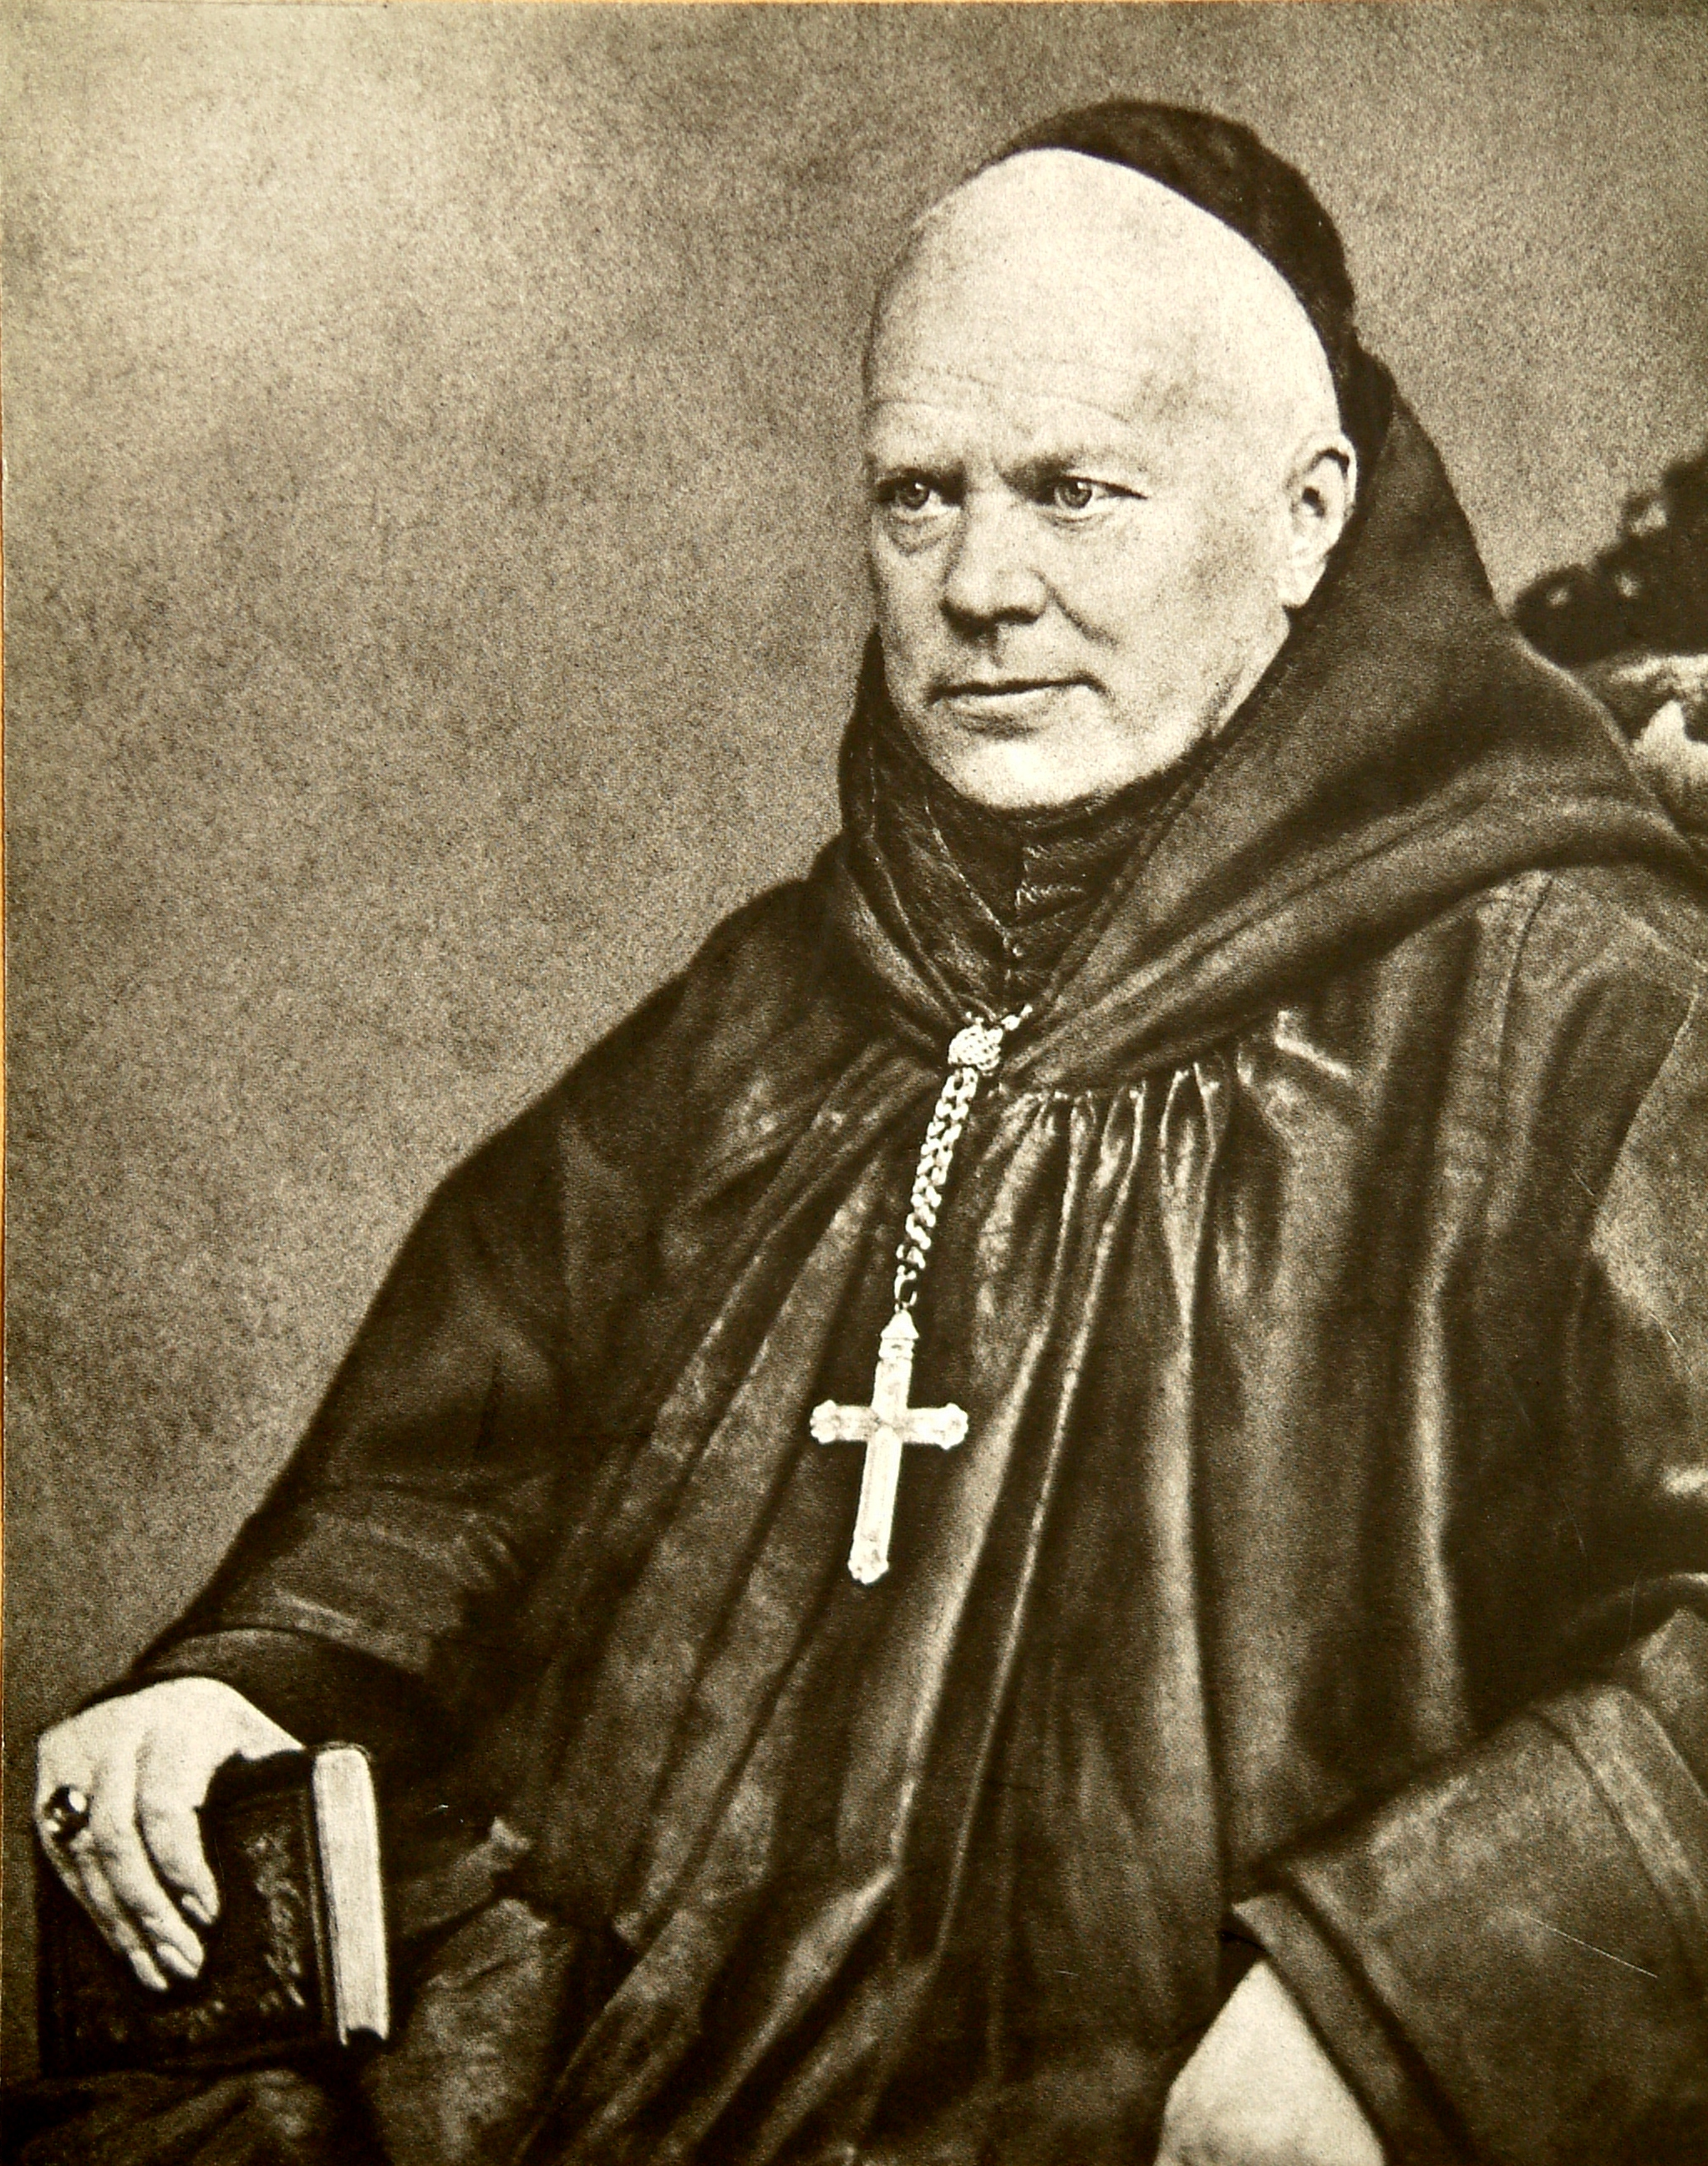
\includegraphics[width=10cm]{dom_gueranger_bath.jpg}
\vspace{2mm}\par
Dom Prosper Guéranger, abbé de Saint-Pierre de Solesmes\par
\end{center}

\pagebreak

Au XXI\textsuperscript{e} siècle, nous devons chercher à être pleinement religieux, c’est-à-dire des êtres qui
contribuent à une union intime entre le ciel et la terre, qui relient le visible et l’invisible, qui
accordent l’esprit et la matière. Donnons à la liturgie l’éclat qu’elle doit avoir, puisqu’elle est la
préfiguration et le commencement de la liturgie céleste. À ce sujet, Dom Guéranger dit ceci de la
poésie et de la liturgie\footnote{\textsc{dom Prosper Guéranger}, Introduction à l’Année liturgique, éd. DMM, 1995, p. 23.}:

\vspace{5mm}


« Dans la liturgie, comme dans les Écritures inspirées, [la poésie] est partout, parce qu’elle seule
est à la hauteur de ce qu’il faut exprimer ; et la collection des monuments de la prière publique, à
mesure qu’elle s’achève, devient aussi le plus riche dépôt de la poésie chrétienne, celle qui chante
sur la terre les mystères du ciel et nous prépare aux cantiques du ciel. »

\vspace{5mm}

La cause de canonisation de Dom Prosper Guéranger est ouverte ; elle progresse à grands pas.
L’année 2025 a été une Année Jubilaire, au cours de laquelle a été célébré le 150ᵉ anniversaire de sa
mort. Il faut prendre Dom Guéranger comme modèle et le prier pour obtenir les grâces dont nous
avons besoin.

\vfill

\emph{« Dieu notre Père, ton serviteur Dom Prosper Guéranger, abbé de Solesmes, attentif à l’Esprit Saint, a permis à une multitude de fidèles de redécouvrir le sens de la liturgie, source du véritable esprit chrétien. Que son dévouement à la Sainte Église et que son amour filial envers la Vierge immaculée, puisés dans le mystère du Verbe incarné, soient une lumière pour les chrétiens de notre temps. Daigne, Seigneur, nous accorder la faveur que nous demandons par son intercession, afin que sa sainteté soit reconnue de tous et que l’Église nous permette au plus tôt de l’invoquer comme l’un de tes bienheureux et de tes saints. Par Jésus, le Christ, notre Seigneur. Amen. »}

\pagebreak

\end{document}